% Standalone pgfplots: the arc's separation ratios (log scale).
% All numbers verbatim from the .verdicts/ ledger. Bar = ratio; horizontal line
% = the frozen V14 bar (1.5). DENSITY axis (NOVEL/REPEAT, H_1203) and the i.i.d.
% trajectory FAIL (NOVEL/SHUFFLED 0.992, H_1203/1207/1208) vs the ORDERED-stream
% trajectory PASS (10.916, H_1208/1209). Sleep persistence 20.7x (H_1204).
\documentclass[border=4pt]{standalone}
\usepackage{pgfplots}
\pgfplotsset{compat=1.18}
\begin{document}
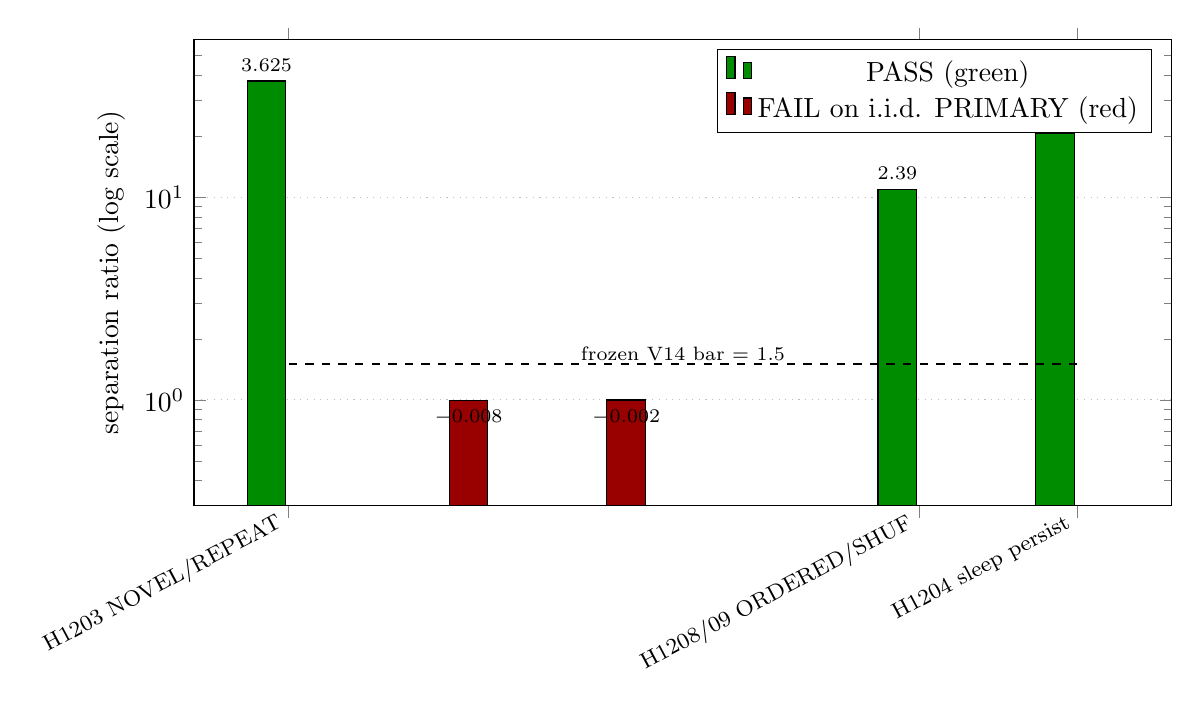
\begin{tikzpicture}
\begin{axis}[
    width=14cm, height=7.5cm,
    ybar,
    bar width=14pt,
    ymode=log,
    log origin=infty,
    ymin=0.3, ymax=60,
    ylabel={separation ratio (log scale)},
    symbolic x coords={
      {H1203 NOVEL/REPEAT},
      {H1203 NOVEL/SHUF (iid)},
      {H1207 recurrent (iid)},
      {H1208 GATE-B (iid)},
      {H1208/09 ORDERED/SHUF},
      {H1204 sleep persist}},
    xtick=data,
    x tick label style={rotate=28, anchor=east, font=\footnotesize},
    nodes near coords,
    nodes near coords style={font=\scriptsize, /pgf/number format/fixed, /pgf/number format/precision=3},
    ymajorgrids, grid style={dotted},
    enlarge x limits=0.12,
]
\addplot[fill=green!55!black] coordinates {
  ({H1203 NOVEL/REPEAT}, 37.538)
  ({H1204 sleep persist}, 20.7483)
  ({H1208/09 ORDERED/SHUF}, 10.916)
};
\addplot[fill=red!60!black] coordinates {
  ({H1203 NOVEL/SHUF (iid)}, 0.992)
  ({H1207 recurrent (iid)}, 0.998)
  ({H1208 GATE-B (iid)}, 0.261)
};
% frozen V14 bar
\draw[dashed, thick, black] (axis cs:{H1203 NOVEL/REPEAT},1.5) -- (axis cs:{H1204 sleep persist},1.5)
  node[pos=0.5, above, font=\scriptsize, fill=white, inner sep=1pt] {frozen V14 bar = 1.5};
\legend{PASS (green), FAIL on i.i.d. PRIMARY (red)}
\end{axis}
\end{tikzpicture}
\end{document}
